\documentclass[a4paper,11pt,exos]{nsi} % COMPILE WITH DRAFT
\usepackage{pifont}
\usepackage{fontawesome5}
\usepackage{hyperref}
\usepackage{pgfplots}


\pagestyle{empty}

\begin{document}
\classe{\terminale Comp}
\titre{Prime d'ancienneté}
\maketitle


Les employés du service informatique d'une entreprise ont reçu des primes différentes selon leur ancienneté. Ils comparent les montants de leurs primes.\\ Leurs observations sont reportées dans le tableau ci-dessous :
\begin{center}
    \tabstyle[UGLiBlue]
    \begin{tabular}{|c|c|c|c|c|c|c|}
    \hline
    \ccell Employé & n°1 & n°2 & n°3 & n°4 & n°5 & n°6  \\\hline
    \ccell Années d'ancienneté & 2 & 8 & 11 & 17 & 20 & 22 \\\hline
    \ccell Prime (en €) & 290 & 390 & 450 & 580 & 640 & 710 \\\hline
    \end{tabular}
\end{center}

Les employés se demandent comment ont été calculées ces primes. Ils ont représenté les points $\pc{M_i}{x_i}{y_i}$ dans un repère orthonormé, où $x_i$ est le nombre d'années d'ancienneté de l'employé $i$ et $y_i$ est le montant de sa prime.
\begin{center}
    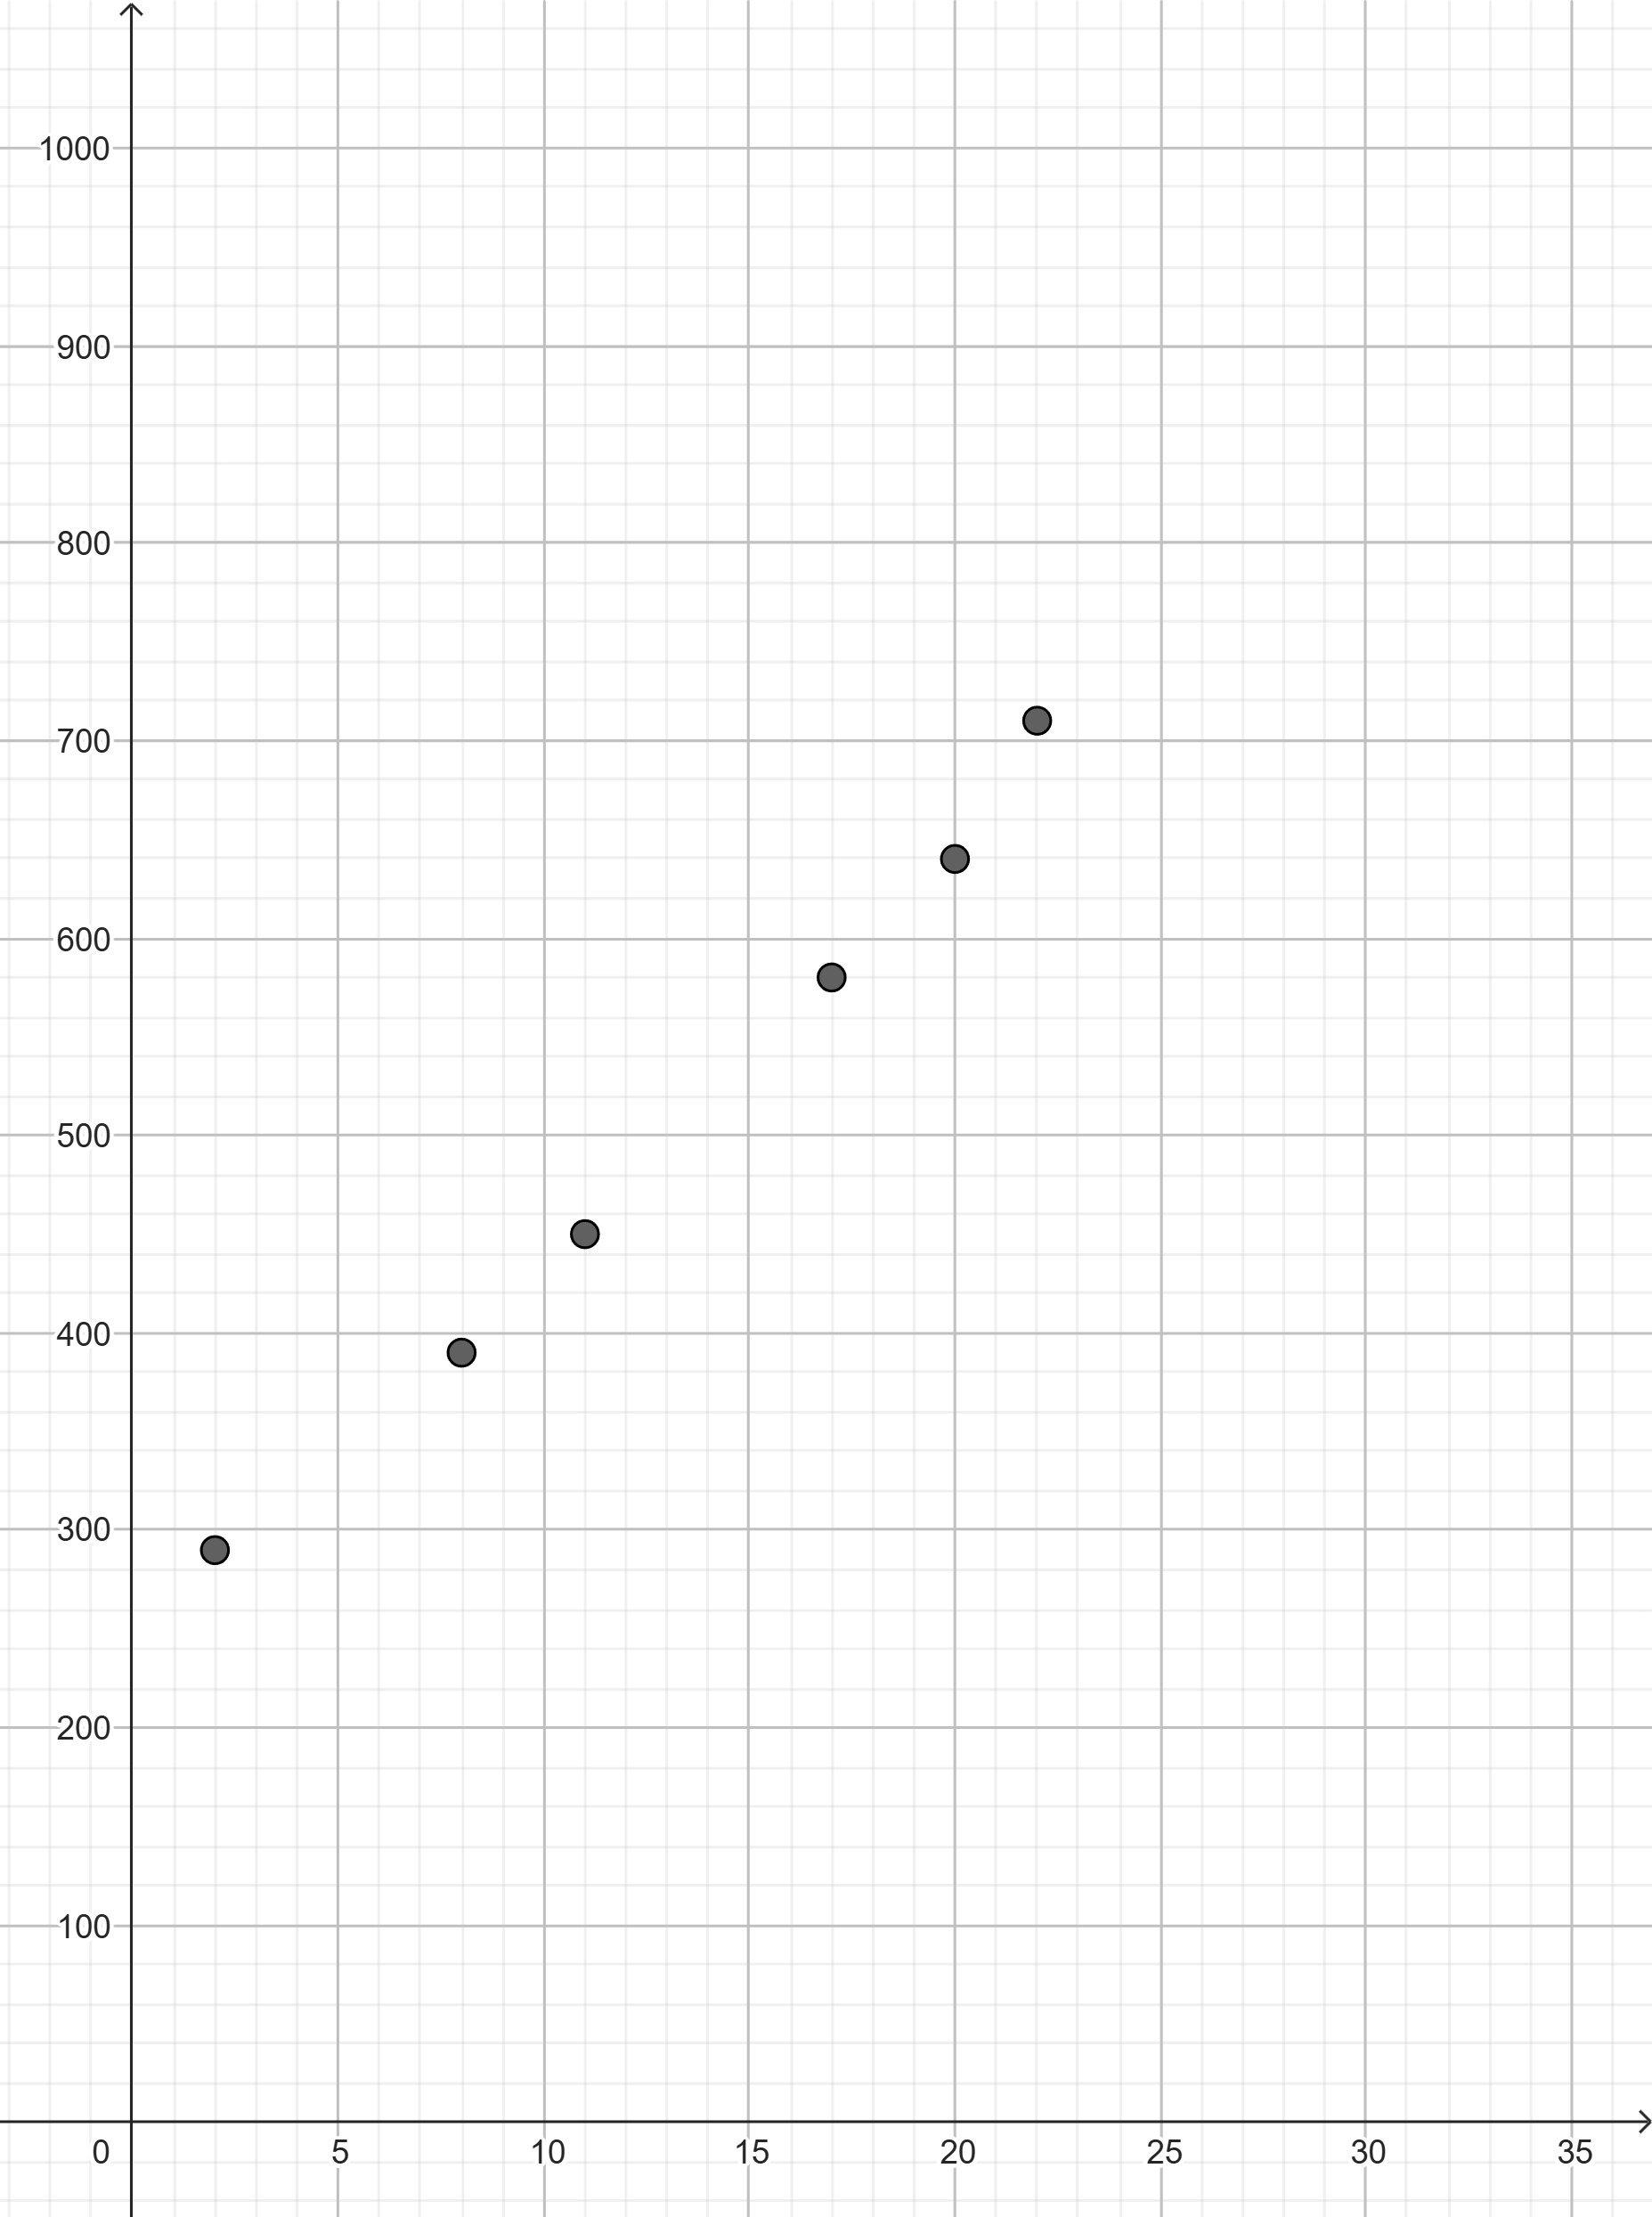
\includegraphics[width=11cm]{Prime.png}
\end{center}
    
Ils se posent les questions suivantes :
    \begin{enumerate}[label=\textbullet]
        \item Quel est l'« employé moyen » de ce service ?
        \item Peut-on prévoir la prime d'un employé avec 15 ans d'ancienneté ? D'un employé débutant ? D'un employé avec 30 ans d'ancienneté ?
    \end{enumerate}


\end{document}